Além da verificação da eficiência dos controladores atuando sobre o sistema para o qual foram projetados, eles foram testados num sistema em que um dos parâmetros foi acrescido de mais de 100 \%, com a massa passando de 2,3 kg para 5 kg.

A resposta dos controladores \textit{fuzzy} e neuro-\textit{fuzzy} para altitude do \textit{drone} nessas circunstâncias são mostradas nas Figuras \ref{fig:altitude_z_zdot_5kg} e \ref{fig:altitude_z_zdot_5kg_closer}, sendo que esta segunda é apenas uma forma melhor de comparar a ação dos dois controladores. Como se pode perceber, ambos os controladores levaram à estabilização do sistema, sendo que desta vez cada um obteve desempenho melhor sob determinados aspectos. No controle da posição vertical $z$, o neuro-fuzzy apresentou tempo de convergência 57\% maior, em parte causado por uma sobrelevação, que não foi apresentada pelo \textit{fuzzy}. Em contrapartida, o neuro-fuzzy apresentou uma menor variação, a reduzindo em 20\% se comparado ao \textit{fuzzy}. Com relação à velocidade $\dot{z}$, o controlador neuro-\textit{fuzzy} apresentou aumento de 23\% no tempo de convergência, mas melhorou o sistema nos quesitos variação e sobrelevação, as reduzindo em 16\% e 33\%, respectivamente. Esses resultados apontam que o quadricóptero, quando submetido ao controle neuro-\textit{fuzzy}, apresentou movimentos mais suaves até ter sua altitude estabilizada, apesar de ter sido necessário mais tempo para que ela ocorresse.

% Altitude m=5
\begin{figure}[!htb]
    \centering
    \caption{Comparação da resposta das saídas $z$ e $\dot{z}$ no controle de altitude \textit{fuzzy} e neuro-\textit{fuzzy} para o sistema com massa $m=5$ kg}
    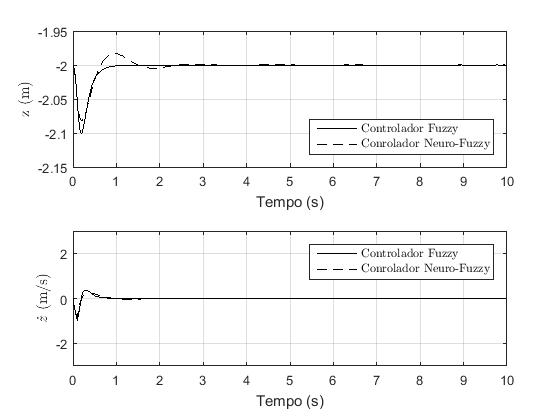
\includegraphics[width=0.8\textwidth]{./04-figuras/figuras_pos_banca/6-altitude5kg/graph_z_zdot_5kg}
    \label{fig:altitude_z_zdot_5kg}
\end{figure}

% Altitude m=5, closer
\begin{figure}[!htb]
    \centering
    \caption{Comparação em mais detalhes da resposta das saídas $z$ e $\dot{z}$ no controle de altitude \textit{fuzzy} e neuro-\textit{fuzzy} para o sistema com massa $m=5$ kg}
    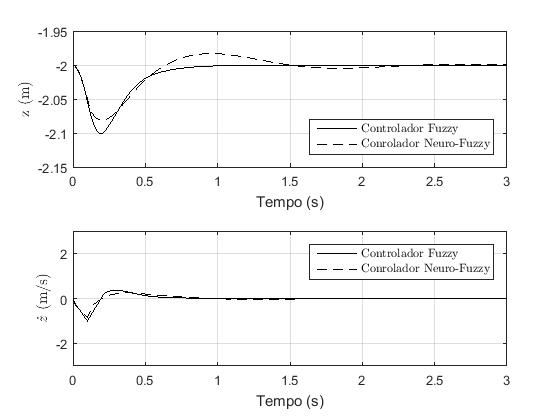
\includegraphics[width=0.8\textwidth]{./04-figuras/figuras_pos_banca/6-altitude5kg/graph_z_zdot_5kg_details}
    \label{fig:altitude_z_zdot_5kg_closer}
\end{figure}


% -------------------  ATITUDE ---------------

Por fim, as Figuras \ref{fig:atitude_phi_phidot_5kg_40s} e \ref{fig:atitude_theta_thetadot_5kg_40s} mostram os resultados obtidos pelos controladores de atitude no sistema com massa $m=5$ kg. Percebe-se que mais uma vez o sistema convergiu ao seu estado de estabilidade com os ângulos nulos e velocidades angulares também nulas, representando que o quadricóptero, após a ação de controle, tanto \textit{fuzzy} quanto neuro-\textit{fuzzy}, fica estável e com orientação plana\footnote{i.e\ paralela ao plano XY}.

As Figuras \ref{fig:atitude_phi_phidot_5kg_10s} e \ref{fig:atitude_theta_thetadot_5kg_10s} mostram em mais detalhes as repostas obtidas pelos controladores sobre a atitude do sistema com massa $m=5$ kg. A partir delas, nota-se que mais uma vez o controlador neuro-\textit{fuzzy} apresentou desempenho levemente superior ao \textit{fuzzy}. Sobre os ângulos $\phi$ e $\theta$, a convergência ocorreu 3\% mais rapidamente e a variação apresentada reduziu 14\%. Já sobre as velocidades angulares $\dot{\phi}$ e $\dot{\theta}$, a redução de tempo de convergência com o neuro-\textit{fuzzy} foi de 2\%, mantendo a mesma sobrelevação e variação oferecidas pelo \textit{fuzzy}. Com isto, mais uma vez o controle neuro-fuzzy fez com que o ângulo máximo de inclinação do \textit{drone} fosse inferior ao alcançado pelo sistema controlado pelo \textit{fuzzy},e além de reduzir o tempo necessário para sua estabilização definitiva.

%phi
\begin{figure}[!htb]
    \centering
    \caption{Comparação da resposta das saídas $\phi$ e $\dot{\phi}$ no controle de atitude \textit{fuzzy} e neuro-\textit{fuzzy} para o sistema com massa $m=5$ kg}
    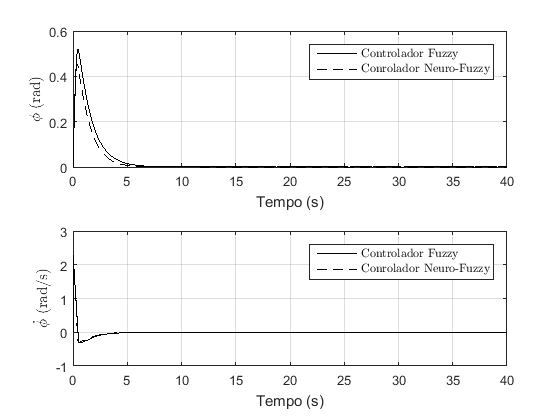
\includegraphics[width=0.8\textwidth]{./04-figuras/resultados/novos/atitude_phi_phidot_5kg_40s}
    \label{fig:atitude_phi_phidot_5kg_40s}
\end{figure}

%theta
\begin{figure}[!htb]
    \centering
    \caption{Comparação da resposta das saídas $\theta$ e $\dot{\theta}$ no controle de atitude \textit{fuzzy} e neuro-\textit{fuzzy} para o sistema com massa $m=5$ kg}
    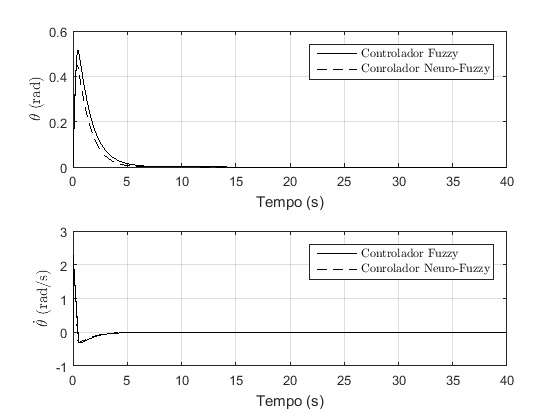
\includegraphics[width=0.8\textwidth]{./04-figuras/resultados/novos/atitude_theta_thetadot_5kg_40s}
    \label{fig:atitude_theta_thetadot_5kg_40s}
\end{figure}

\begin{figure}[!htb]
    \centering
    \caption{Comparação da resposta das saídas $\phi$ e $\dot{\phi}$ no controle de atitude \textit{fuzzy} e neuro-\textit{fuzzy} para o sistema com massa $m=5$ kg}
    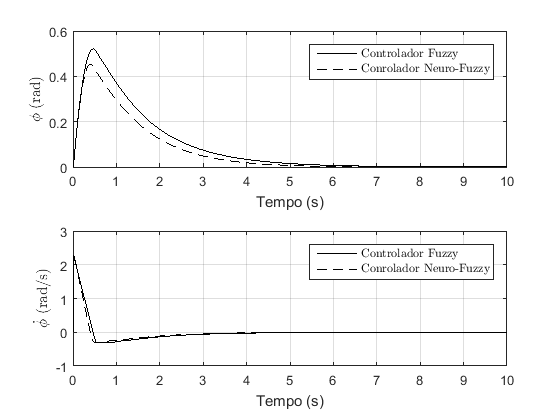
\includegraphics[width=0.8\textwidth]{./04-figuras/resultados/novos/atitude_phi_phidot_5kg_10s}
    \label{fig:atitude_phi_phidot_5kg_10s}
\end{figure}

%theta
\begin{figure}[!htb]
    \centering
    \caption{Comparação da resposta das saídas $\theta$ e $\dot{\theta}$ no controle de atitude \textit{fuzzy} e neuro-\textit{fuzzy} para o sistema com massa $m=5$ kg}
    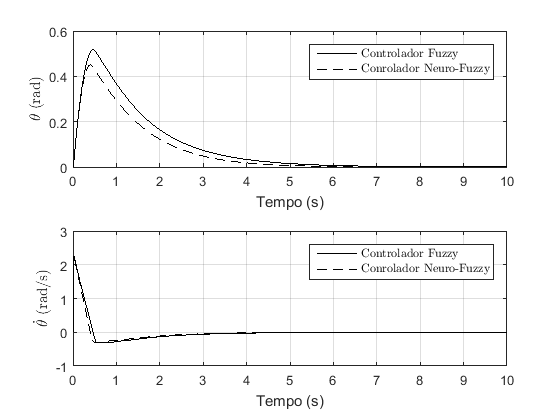
\includegraphics[width=0.8\textwidth]{./04-figuras/resultados/novos/atitude_theta_thetadot_5kg_10s}
    \label{fig:atitude_theta_thetadot_5kg_10s}
\end{figure}




